% Author: PokMan Ho
% Script: res_prep.tex
% Desc: result section preparation
% Input: none
% Output: none
% Arguments: 0
% Date: Jun 2020

\documentclass[../thesis.tex]{subfiles} %% use packages & commands as this main file

\begin{document}

\section{Distributions}
\begin{figure}[H]
    \centering
    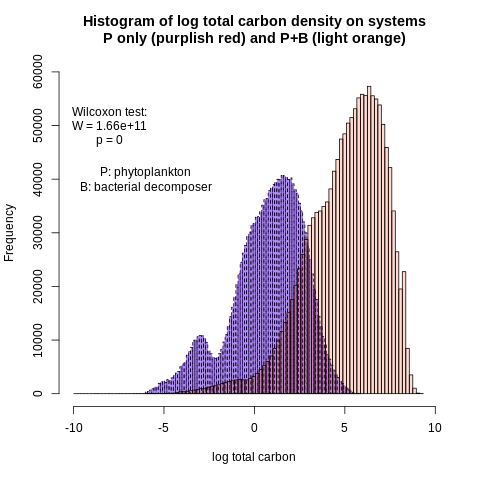
\includegraphics[width=.7\linewidth]{report/media/hist_PvsPB_A.png}
    \caption{Histogram of distribution on sustainable yield for total carbon in the system across the whole parameter space}
    \label{hist:A}
\end{figure}

Fig.\ref{hist:A} is the distribution of sustainable yield between the equilibrium position between phytoplankton only [P] and phytoplankton \& bacterial decomposer [P+B] set-ups.
\begin{itemize}
    \item both distributions are not normally-distributed $\rightarrow$ non-parametric test
    \item Wilcox-test: significantly different
    \item P+B $>$ P
\end{itemize}

Criticism: is the difference only due to the incorporation of bacterial biomass?
\begin{itemize}
    \item org-C: P+B $<$ P (Fig.\ref{hist:C})
    \item org-P: P+B == P (by eqm position calculation)
    \item org-B: P+B $>$ 0, P == 0 (by definition, P-only setting has no bacteria)
\end{itemize}
The figure not only indicated the effect by incorporating B, but also the reduction of org-C due to the carbon processing by B.  Yet the overall effect is still making P+B $>$ P in overall carbon in log-scale

\begin{figure}[H]
    \centering
    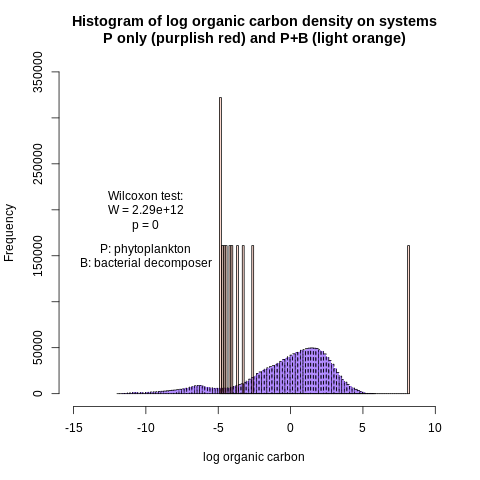
\includegraphics[width=.7\linewidth]{report/media/hist_PvsPB_C.png}
    \caption{Histogram of distribution on sustainable yield for organic carbon pool across the whole parameter space}
    \label{hist:C}
\end{figure}

Criticism: why do the distribution in ``total carbon" choppy?

\begin{figure}[H]
    \centering
    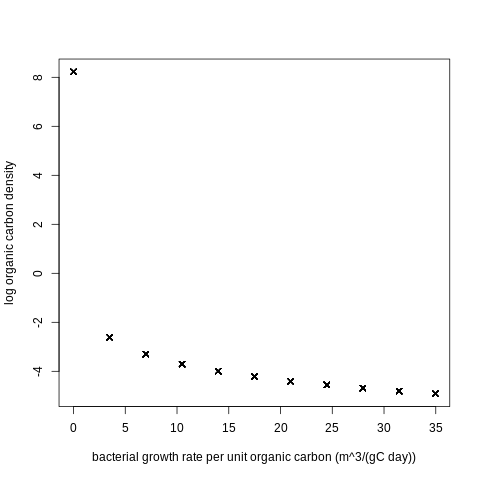
\includegraphics[width=.5\linewidth]{report/media/gBEffectOnOrgC.png}
    \caption{Plot of log organic carbon density against bacterial growth rate per unit organic carbon density ($\frac{m^3}{gC\cdot day}$)}
    \label{fig:orgCVSgB}
\end{figure}

From Fig.\ref{fig:orgCVSgB}, $\gB$ determined the result for organic carbon.  It is because the organic carbon fraction analytical solution is different between the two systems.  In equilibrium position 3, the organic carbon pool is totally related to parameters by phytoplankton while in co-existence solution the pool is completely relying on bacterial parameters.  Since in the parameter space scanning all bacterial parameters except $\gB$ has only one value (while $\gB$ is scanned with regular interval within a range), the distribution is logically deterministic and looks uniform and governed by $\gB$.

\begin{table}[H]
    \centering
    \caption{Table showing analytical solved possible equilibrium solutions from the ODE model}
    \begin{tabular}{c|ccc}\hline
        & C & P & B\\\hline
        eqm1 & 0 & 0 & 0\\
        eqm2 & $\frac{\mB}{\eBR\eB\gB}$ & 0 & $\frac{x}{\gB(\eBR-1)}$\\
        eqm3 & $\frac{\eP(\ePR\gP)^2}{\aP x}$ & $\frac{\ePR\eP\gP}{\aP}$ & 0\\
        eqm4 & $\frac{\mB}{\eBR\eB\gB}$ & $\frac{\ePR\eP\gP}{\aP}$ & $\frac{\aP\mB x-\eBR\eB\gB\eP(\ePR\gP)^2}{\aP\mB\gB(\eBR-1)}$\\\hline
    \end{tabular}
    \label{tab:anaSol}
\end{table}

\section{realistic parameter combinations}
\begin{itemize}
    \item yield flux (i.e.$xC$ term in equation, $\frac{gC}{m^3\text{day}}$) distribution:
\end{itemize}
\begin{center}
    \begin{tabular}{c|ccccccccccc}\hline
        \% & 0 & 10 & 20 & 30 & 40 & 50 & 60 & 70 & 80 & 90 & 100\\
        approx flux & 0 & 1e-3 & 3e-3 & 7e-3 & 1e-2 & 2e-2 & 9e-2 & 0.5 & 1.8 & 6.1 & 3700\\\hline
    \end{tabular}
\end{center}
\begin{itemize}
    \item unique parameter behaviour
    \begin{itemize}
        \item $x$ = 0 $day^{-1}$ is not in the maxed out yield, and it is invalid using this model when considering P-only situation (as $x$ is at the denominator in eqm3-C density; Table \ref{tab:anaSol})
        \item $\gB$ = 6.9e-5 $\frac{m^3}{gC\cdot day}$ is the only value causing maxed out yield
    \end{itemize}
    \item other parameters are having their whole range also included in this explosive output
\end{itemize}

\section{carbon sequestration limiting factors}

\section{non-independent parameters search}
\begin{itemize}
    \item $\ePR$ is dependent on $\gP$, and range of $\ePR$ used in the model was based on the range of $\gP$ under the same temperature range
    \item 
\end{itemize}

\end{document}
